% Package obligatoire : type de document
\documentclass[a4paper,12pt,twoside]{book}

% Encodage
\usepackage{fontspec}

% Annexes (à déclarer avant hyperref)
\usepackage{appendix}

% Le package hyperref avec des options, si en local
\usepackage[pdfusetitle, pdfsubject ={Mémoire TNAH}, pdfkeywords={les mots-clés}]{hyperref}

% Langues
\usepackage[english,french]{babel}
% Commande personnalisée pour la typographie des langues
\newcommand{\langue}[1]{\emph{#1}}

% Configurer le document selon les normes de l'école
\usepackage[margin=2.5cm]{geometry} % marges
\usepackage{setspace} % espacement qui permet ensuite de définir un interligne
\onehalfspacing % interligne de 1.5
\setlength\parindent{1cm} % indentation des paragraphes à 1 cm

% Table des matières
\addto\captionsfrench{
\renewcommand*\contentsname{Contenu de la documentation}
}
\usepackage[nottoc]{tocbibind}% Pour ajouter la biblio à la TDM sans numérotation de chapitre

% Bibliographie
\usepackage[backend=biber, sorting=nyt, style=enc,maxbibnames=10]{biblatex}
\addbibresource{./biblio.bib}

%\nocite{*}

% Sigles et acronymes
\usepackage[automake,acronym,toc]{glossaries}
\makeglossaries
\newacronym{bnf}{BnF}{Bibliothèque nationale de France}
\newacronym{cds}{CdS}{Constance de Salm}
\newacronym{cg2c2v}{Corr.~g., 2e copie, 2e vol.}{long}
\newacronym{cremma}{Cremma}{Consortium Reconnaissance d’Écriture Manuscrite des Matériaux Anciens}
\newacronym{dahn}{DAHN}{Digital Edition of historical manuscripts}
\newacronym{dhi}{DHIP}{Deutsches Historisches Institut Paris}
\newacronym{enc}{ENC}{École nationale des chartes}
\newacronym{fud}{FuD}{Die Virtuelle Forschungsumgebung für die Geistes- und Sozialwissenschften}
\newacronym{htr}{HTR}{\textit{Handwritten Text Recognition}}
\newacronym{lectaurep}{Lectaurep}{Lecture Automatique de Répertoires}
\newacronym{Segmonto}{SegmOnto}{SegmOnto~: A Controlled Vocabulary to Describe the Layout of Pages}

% Images
\usepackage{graphicx}

% Citations
\usepackage{csquotes}

% Blocs de code
%\usepackage{minted}% [cache=false] fait disparaître le message d'erreur mais le contenu ne s'affiche plus

% Schéma d'arborescence de dossiers
\usepackage[edges]{forest}
\usepackage{array}
\definecolor{folderbg}{RGB}{124,166,198}
\definecolor{folderborder}{RGB}{110,144,169}
\newlength\Size
\setlength\Size{4pt}
\tikzset{%
	folder/.pic={%
		\filldraw [draw=folderborder, top color=folderbg!50, bottom color=folderbg] (-1.05*\Size,0.2\Size+5pt) rectangle ++(.75*\Size,-0.2\Size-5pt);
		\filldraw [draw=folderborder, top color=folderbg!50, bottom color=folderbg] (-1.15*\Size,-\Size) rectangle (1.15*\Size,\Size);
	},
	file/.pic={%
		\filldraw [draw=folderborder, top color=folderbg!5, bottom color=folderbg!10] (-\Size,.4*\Size+5pt) coordinate (a) |- (\Size,-1.2*\Size) coordinate (b) -- ++(0,1.6*\Size) coordinate (c) -- ++(-5pt,5pt) coordinate (d) -- cycle (d) |- (c) ;
	},
}
\forestset{%
	declare autowrapped toks={pic me}{},
	pic dir tree/.style={%
		for tree={%
			folder,
			font=\itshape,
			grow'=0,
		},
		before typesetting nodes={%
			for tree={%
				edge label+/.option={pic me},
			},
		},
	},
	pic me set/.code n args=2{%
		\forestset{%
			#1/.style={%
				inner xsep=2\Size,
				pic me={pic {#2}},
			}
		}
	},
	pic me set={directory}{folder},
	pic me set={file}{file},
}
\newcommand{\fname}[2]{\begin{tabular}{m{1cm}@{\quad}m{4cm}}#1 & \normalfont#2\end{tabular}}

% DOCUMENT
\begin{document}
	
	\tableofcontents
	
	\chapter*{Présentation}
	\addcontentsline{toc}{chapter}{Présentation}% Ajoute à la table des matières sans numérotation
	
		\section*{Contexte}
		\addcontentsline{toc}{section}{Contexte}
		Constance de Salm (1767-1845), femme de lettres française, a entretenu une vaste correspondance à partir de son mariage avec de nombreux intellectuels en Allemagne, en France, en Russie.

		Le projet de publier numériquement sa correspondance est né de l'intérêt pour les relations entre noblesses française et allemande au sein du \gls{dhi}. Il en a résulté la production d'un site \textit{Wordpress} adossé au système de base de données \href{https://fud.uni-trier.de/}{\gls{fud}}. Les notices de plus de 11000 lettres, publiées sur le site \href{https://constance-de-salm.de}{constance-de-salm.de}, associent la reproduction numérique des documents manuscrits (lettres, copies, brouillons, recueils) avec leurs métadonnées descriptives, ainsi qu'une transcription de la première ligne de chaque lettre.

		\section*{Objectifs}
		\addcontentsline{toc}{section}{Objectifs}
		L'objectif du stage consiste à mettre en place un flux de production automatisé pour l'édition des lettres au format XML-TEI. On s'appuiera pour cela sur les instruments et la documentation produits dans le cadre du projet \gls{dahn}, fondé sur l'édition de la correspondance de Paul d’Estournelles de Constant (1852-1924)\footcite{chiffoleauDAHNProject}.
		
		Il s'agit en particulier d'identifier les points de difficultés que posent le traitement de ce vaste corpus tant du point de vue de la transcription automatisée des documents que du point de vue de leur encodage au format TEI. 
		
		Il serait notamment souhaitable, au terme du stage de disposer d'un flux de production pour l'édition d'un volume de recueil de lettres.
			
	\chapter{Reconnaissance automatique des écritures manuscrites}
		
		\section{Problématique}
			
			\subsection{Des sources écrites par plusieurs mains}
				Quatre à cinq mains différentes ont été repérées jusqu'à présent dans la correspondance de \gls{cds} (mais aucune enquête paléographique complète n'a été menée). Cette variété des écritures est un problème majeur pour l'automatisation des transcriptions.
				
				Les choix effectués dans le cadre du projet \gls{lectaurep} ont permis de guider notre démarche. L'alternative méthodologique a été décrite ainsi par A.~Chagué~:
				
				\begin{quotation}
					Quand on se lance dans une campagne de transcription reposant sur la reconnaissance d’écritures manuscrites, on passe généralement par une série de questions qui sont les mêmes d’un projet à l’autre. Parmi ces questions, il y a celle des modèles de transcription et de leur rapport à la variation des écritures. Doit-on entraîner un modèle pour chaque type d’écriture présent dans un corpus de documents~? Au contraire, peut-on se contenter d’entraîner un seul modèle tout terrain (qu’on appellera mixte ou générique)~?\footcite{chagueCreationModelesTranscription}
				\end{quotation}
			
				Les résultats probants obtenus par le projet \gls{lectaurep} en suivant l'option d'entraînement d'un modèle mixte\footcite{chagueCreationModelesTranscriptiona} nous ont convaincu d'emprunter cette voix.
			
				Deux séries de tests méritaient dès lors d'être effectuées~:
		
				\begin{enumerate}
					\item Reprendre les tests sur le modèle entraîné de zéro par H.~Souvay lors d'un précédent stage consacré à la correspondance de \gls{cds}\footcite{souvayCorrespondanceConstanceSalm2021}~;
					\item Reprendre un modèle générique entraîné pour le projet \gls{lectaurep} .
				\end{enumerate}
		
			\subsection{Objectif~: éditer}
				Il faut prendre en considération dans les choix méthodologiques du processus d'\gls{htr} les objectifs à atteindre. Il s'agit d'éditer le texte en restant proche de l'usage scribal, sans donc le corriger~:
				
				\begin{enumerate}
					\item La transcription ne résout pas les abréviations~;
				\end{enumerate}
				
		\section{Choisir des collections d'évaluation}
			Afin de donner les meilleurs chances aux tests à effectuer avec le modèle entraîné par H.~Souvay, nous sommes repartis des mêmes vérités de terrain, issues de la seconde copie de la correspondance générale. Ces recueils de lettres constituent la part du corpus la plus normée sur le plan de l'écriture et de la mise en page, leur qualité de conservation assurant en outre de bonnes conditions à la reconnaissance d'écriture. Nous avons particulièrement exploité les trois premiers volumes de cet ensemble qui en compte six\footnote{\cite{salmCorrespondanceGeneraleSecondea}~; \cite{salmCorrespondanceGeneraleSeconde}~; \cite{salmCorrespondanceGeneraleSecondeb}.}.
			
			La variété des écritures se partage de manière contrastée entre des mains dominantes et des mains rares. Généralement, deux mains dominantes se partagent un recueil~; leur distribution peut être discontinue. Quant aux mains rares, elles n'occupent que quelques feuillets par recueil~; nous ne les avons pas retenu pour les tests.
			
			Nous avons également analysé les écritures du recueil de la correspondance adressée par J.P.E.~Martini à \gls{cds} afin d'élargir la variété de notre corpus de tests. Nous y avons distingué deux mains\footnote{Une présentation des mains peut être parcourue sur le \href{https://github.com/sbiay/CdS-edition/tree/main/htr/sources}{dépôt du projet}}.
			
			On a privilégié pour les corpus de test et d'entraîner des modèles des reproductions favorables à une bonne reconnaissance de l'écriture, évitant en particulier les problèmes de transparence qui font ressortir au recto l'encre du verso.
					
			Concernant l'écriture personnelle de \gls{cds}, le site ne publie aucune lettre originale de sa main, mais 52 brouillons (\textit{Entwurf}). Entraîner un modèle de reconnaissance sur cette écriture suppose un travail délicat de transcription pour une écriture particulièrement cursive (compter environ deux semaines pour disposer d'une bonne vingtaine de pages).
		
		\section{Préparer le traitement d'un dossier}
			L'archive photographique de la correspondance de Constance de Salm comporte des documents non inventoriés. Afin de n'engager dans notre chaîne de traitement que des documents effectivement inventoriés, nous avons consacré un \textit{notebook} à la préparation du traitement d'un dossier\footcite{biayPreparerTraitementDossier2022}.
			
			Après l'étape préliminaire de l'import local et de la conversion des images au format Jpeg (afin de ne pas travailler avec le format Tiff, trop lourd), il est nécessaire d'établir la liste des images associées à une notice de l'inventaire. Nous avons pour cela écrit un script python\footcite{biayDonneesImagesPy2022} qui analyse les noms des fichiers convertis et importés localement, croise ces noms avec les données de l'inventaire et écrit en sortie un fichier Json qui liste (entre autres informations), pour chaque notice l'inventaire contenant l'une des images du dossier, l'URL de cette notice sur le site \url{https://constance-de-salm.de} et la liste complète des images attachées à cette notice\footnote{Le fichier donne par ailleurs la liste des images qui ne sont liées à aucune notice de l'inventaire ainsi, ainsi qu'une présentation des mêmes données d'association image-notice, mais cette fois par image et non par notice, et ce afin de permettre le contrôle visuel des zones de texte à transcrire (cf.~\textit{infra}, \ref{controle-segmentation-lettres-inventoriees}, p.~\pageref{controle-segmentation-lettres-inventoriees})}.
			
			Une fois le dossier analysé et le fichier produit, les commandes que nous avons écrites dans le \textit{notebook} permettent de n'importer dans le dossier de travail que les images correspondant à une notice de l'inventaire.
			
		\section{Choisir une application~: Transkribus ou eScriptorium~?}
			Au moment de notre stage, les deux principales applications permettant de procéder à la transcription automatique des écritures manuscrites sont eScriptorium et Transkribus.
			
			Différentes considérations peuvent conduire à opter pour l'une ou l'autre de ces applications\footnote{Nous avons assisté le 9 mai 2022 à l'atelier organisé au sein du Data-Lab de la \gls{bnf} et dont le programme est détaillé dans le billet d'\cite{jacquotTranskribusEScriptoriumTranscrire}.}. Le facteur nous apparaissant le plus déterminant a trait aux compétences d'ingénierie des personnes chargées de mener la campagne de transcription.
			
			L'écosystème applicatif Transkribus est celui qui propose le plus grand choix de services, tant pour les utilisateurs ayant des compétences d'ingénierie élevées (logiciel Expert Client) que pour les néophytes (Transkribus Lite). Conjuguées à la facilité de prise en main de Transkribus Lite, les fonctionnalités de gestion des versions de transcription offertes par Transkribus Expert Client rendent cet écosystème le mieux à même d'héberger des campagnes de transcription de grande ampleur, faisant appel à de multiples transcripteurs, voire à de la production participative (ou \textit{crowdsourcing}).
			
			L'application eScriptorium, à un stade de développement moins avancé, avec une interface dotée de moins de fonctionnalités que Transkribus (gestion des versions de transcription, annotation du texte), mobilise davantage de compétences d'ingénierie. En revanche, la gratuité totale de son utilisation et, qui plus est, la culture de science ouverte portée par la communauté qui développe et utilise eScriptorium (ouverture des données de modèles, de vérités de terrain, développement d'outils auxiliaires à la transcription, à la gestion de fichiers, propositions de standards d'annotation) rendent cette application tout à fait adéquate aux projets impliquant un petit nombre de transcripteurs ayant une bonne culture d'ingénierie au préalable, notamment au sein d'institutions désireuses de promouvoir la science ouverte.
			
			Nous avons opté pour eScriptorium dans le cadre de ce stage en raison du dynamisme de la communauté eScriptorium au sein de l'\gls{enc} (à travers le projet \gls{cremma}).

			Nous avons testé son utilisation à partir d'une installation locale, faisant appel aux seules ressources d'un ordinateur portable, à savoir sans serveur ni carte graphique externe. Cette méthode nous a permis de procéder à des entraînements de modèle à partir de petits volumes de vérités de terrain. Si des entraînements plus massifs s'avéraient nécessaires, il serait alors impératif de se tourner vers une infrastructure dotée de plus grandes capacités de calcul, ce que, par exemple, un partenariat entre le \gls{dhi} et le projet \gls{cremma} rendrait possible.
				
		\section{Annoter les régions et les lignes d'écriture}
			L'annotation des régions et des lignes d'écritures répond à deux fonctions distinctes~:
			
			\begin{itemize}
				\item Permettre l'entraînement d'un modèle de segmentation~;
				\item Transformer leur contenu afin de l'affecter à des éléments déterminés de l'arborescence XML-TEI qu'il faudra construire\footnote{C'est aussi un enjeu central du projet \textbf{Galli(corpor)a}}.
			\end{itemize}

				Cette réflexion sur les besoins de la transformation vers le format TEI a été nourrie par les \textit{Guidelines} de l'édition de correspondance du projet DAHN\footcite{chiffoleauCorrespondenceGuidelines2022}. Par ailleurs, F.~Chiffoleau a formulé une ontologie pour les régions et lignes des écrits de correspondance en langue française pour le XXe siècle \footcite{chiffoleauCorrespondanceLangueFrancaise2021} dans le cadre du projet \gls{Segmonto}\footcite{gabaySegmOntoCommonVocabulary2021}. Afin de rendre notre propre typologie générique et de pouvoir exploiter l'outil de validation d'annotation HTRUC\footcite{clericeHTRUCHTRUnitedCatalog2021}, nous avons repris les types \gls{Segmonto} en exploitant les types \texttt{CustomZone} et \texttt{CustomLine} lorsqu'il était nécessaire de les personnaliser.

			\subsection{Régions}
				L'entraînement d'un modèle de segmentation à reconnaître et annoter automatiquement des types de régions d'écritures est un travail complexe. La mise en page des lettres répond à des principes clairs pour l'oeil humain~; il présente en revanche d'importantes variations métriques dans l'espace de la page. Le meilleur exemple de ces variations se trouve dans les recueils~: les lettres ont été transcrites les unes à la suite des autres~; un début de lettre peut dès lors se trouver à n'importe quelle hauteur de la page. 
				
				\textbf{Ajouter un commentaire sur l'espacement des lignes de l'en-tête}
				
				\begin{figure}[!h]
					% !h ancre l'image dans le flux de texte
					\centering
					\includegraphics[scale=0.65]{./img/CdS02_Konv002-02_0193-detail-01.jpg}%
					\caption{Début d'une lettre présentant une disposition aérée des éléments (\cite{salmCorrespondanceGeneraleSeconde}).}%
					\label{}%
				\end{figure}
			
				\begin{figure}[!h]
					% !h ancre l'image dans le flux de texte
					\centering
					\includegraphics[scale=0.65]{./img/CdS02_Konv002-02_0046-detail.jpg}%
					\caption{Début d'une lettre présentant une disposition resserrée des éléments (\cite{salmCorrespondanceGeneraleSeconde}).}%
					\label{}%
				\end{figure}
				
				La reconnaissance de la fin d'une lettre (dont la signature alignée à droite de la page est le premier mais non le seul élément) est encore plus délicate, car elle ne se manifeste jamais par un élément visuellement massif comme un titre.
				
				En raison de cette complexité, nous avons opté pour une typologie de régions resserrée. Tandis que l'ontologie de F.~Chiffoleau proposait un type de région pour chaque élément significatif de l'écrit de correspondance\footcite{chiffoleauCorrespondanceLangueFrancaise2021}, nous n'avons retenu que trois types de régions principaux pour annoter la structure des lettres~:
				
				\begin{itemize}
					\item \textbf{MainZone}~: pour le corps du texte~;
					\item \textbf{CustomZone:opener}~: pour l'en-tête des lettres~;
					\item \textbf{CustomZone:closer}~: pour la clôture des lettres.
				\end{itemize}
			
				\textbf{la définition des régions est formelle, visuelle}
			
			La figure \ref{typageRegions} \hyperref[typageRegions]{ci-dessous} propose une mise en oeuvre de ce typage des régions.	
			
			\begin{figure}[!h]
				% !h ancre l'image dans le flux de texte, sinon elle va n'importe où !
				\centering
				\rotatebox{90}{%
					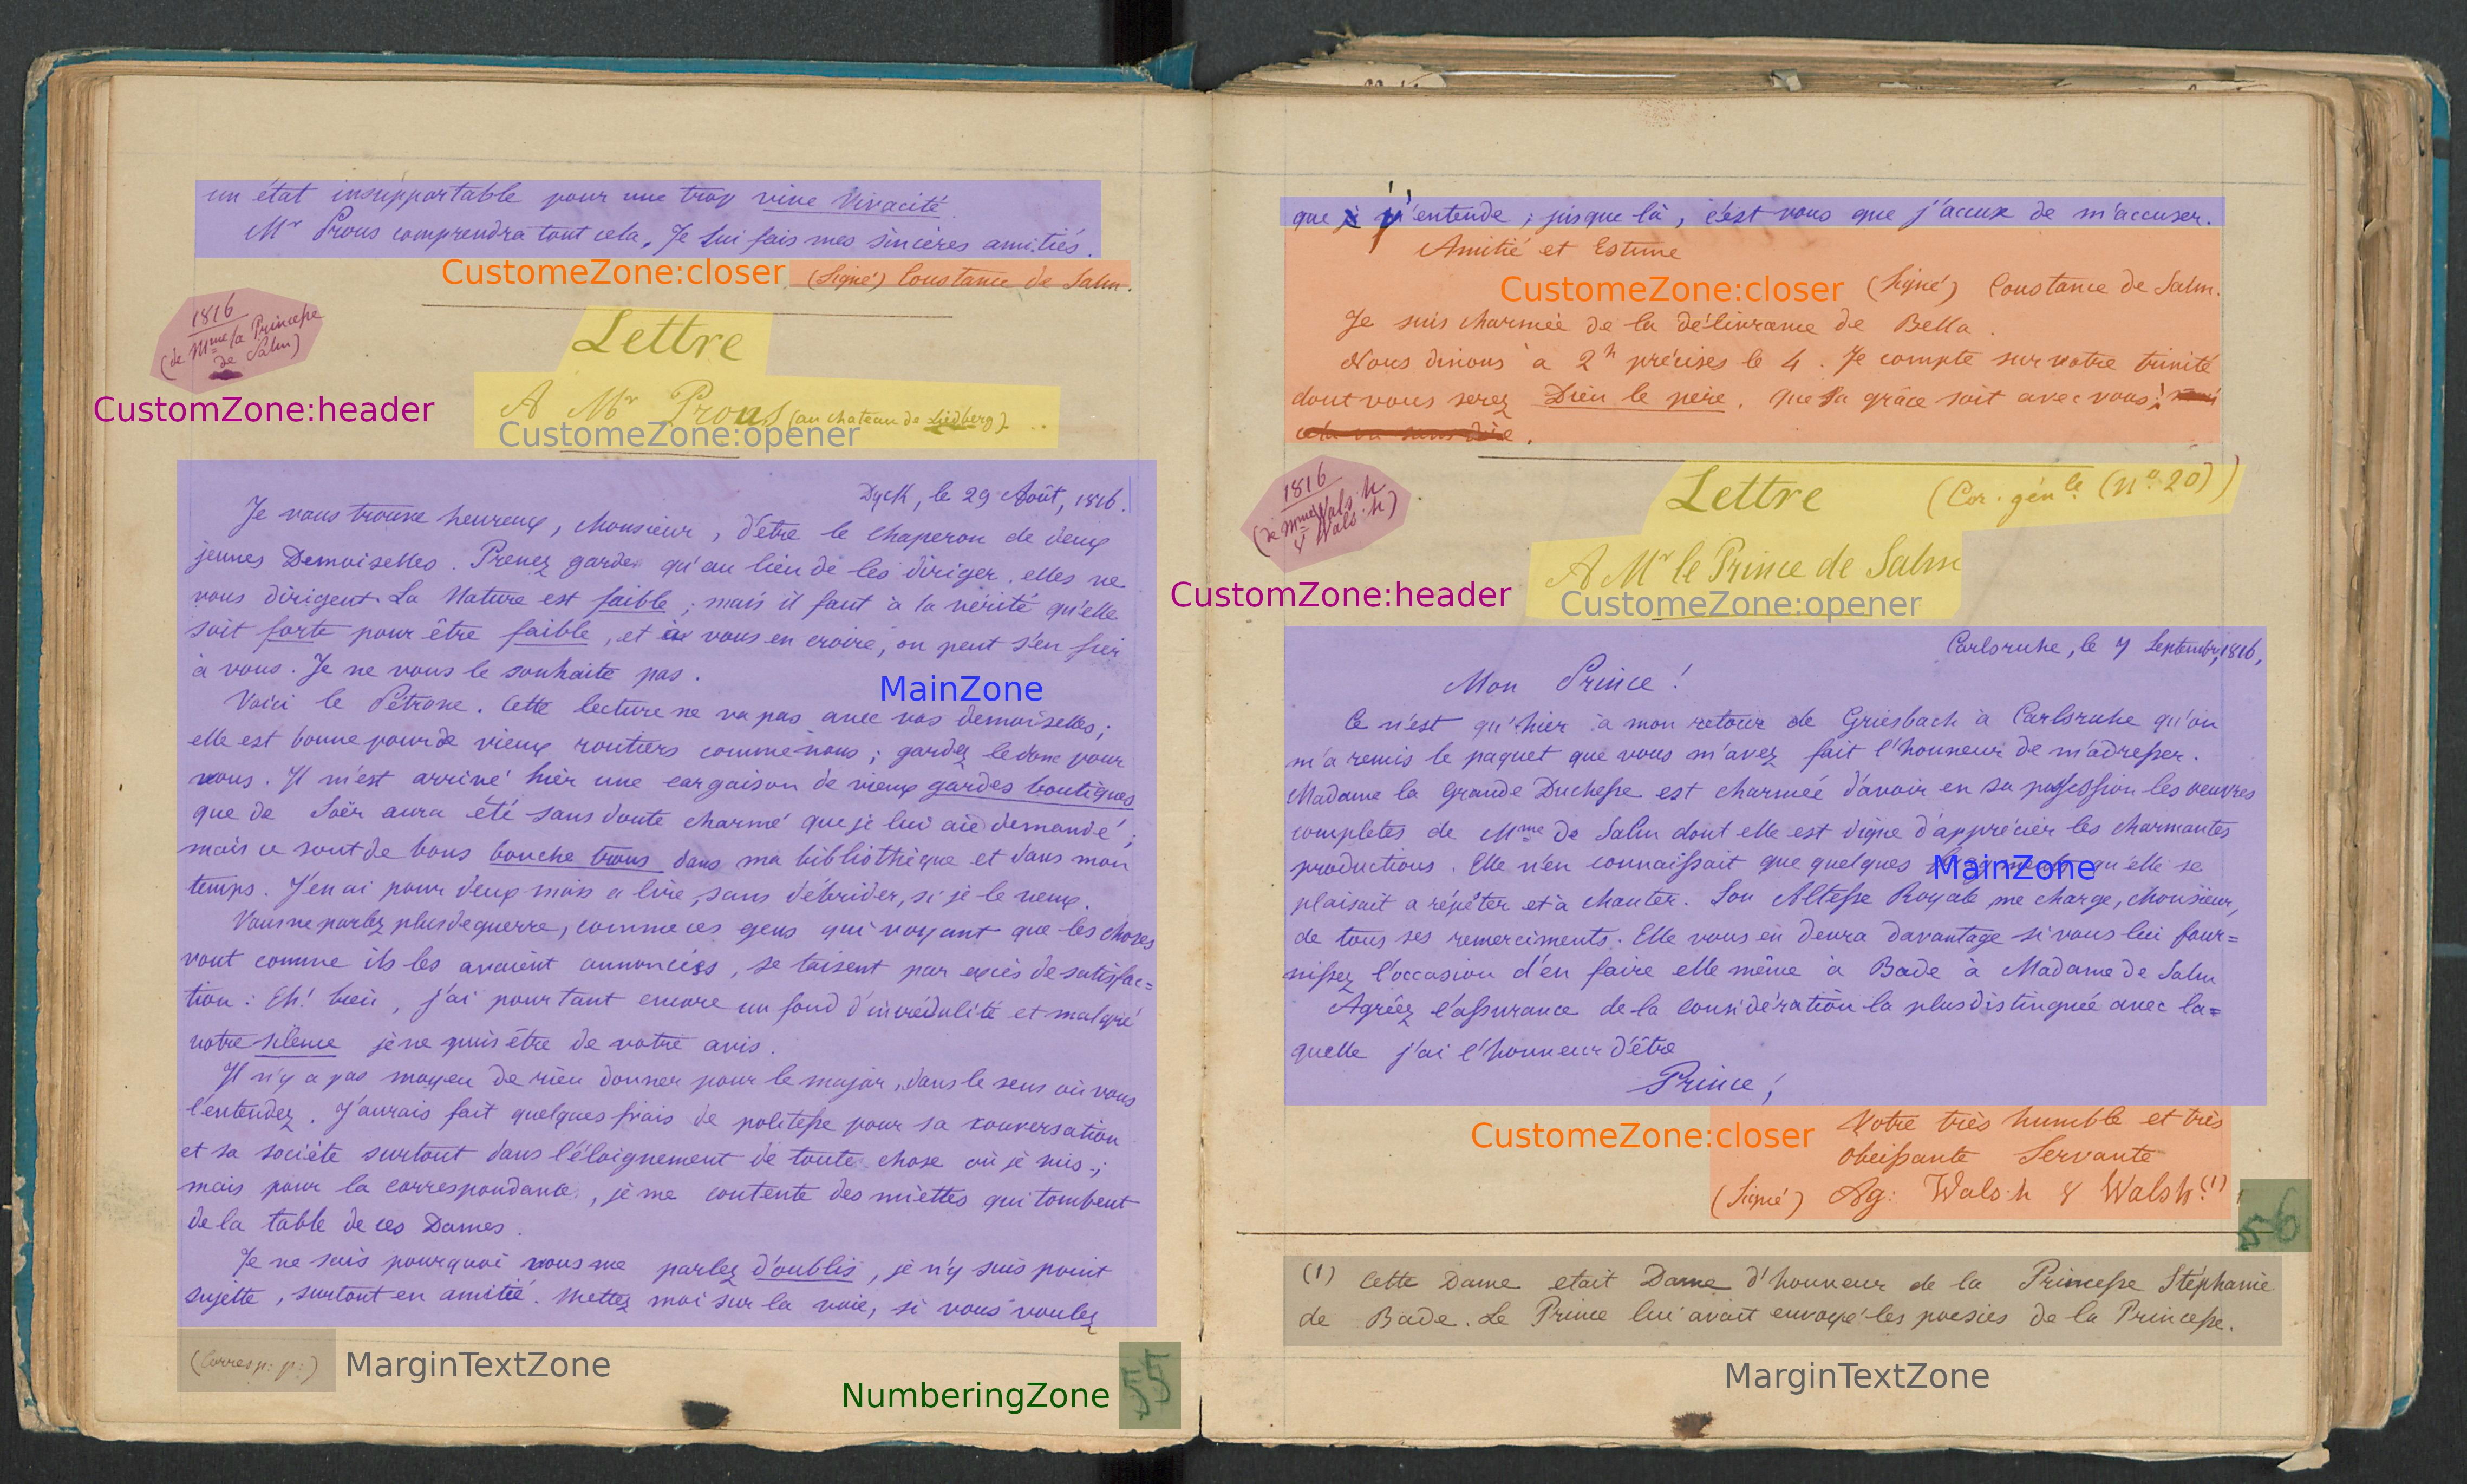
\includegraphics[scale=0.65]{../htr/demo/annotation-CdS02_Konv002-02_0066.png}%
				}%
				\caption{Exemple de typage des zones de texte sur une double page.}%
				\label{typageRegions}%
			\end{figure}
			
			\subsection{Lignes d'écriture}
				Les types de lignes dont on propose l'utilisation sont~:
						
			\subsection{Phénomènes graphiques particuliers}
				\gls{cds} a corrigé certains mots de sa main~:
			
				\begin{itemize}
					\item En rayant une lettre, un mot ou plusieurs mots, ou bien en réécrivant par dessus le texte. Dans de nombreux cas cela consiste en une simple lettre barrée~; le typage de la ligne demanderait alors beaucoup d'effort pour un résultat minime~;
					\item En réécrivant dans l'interligne~: il est alors pertinent d'utiliser le type de ligne e-Scriptorium \textbf{Correction}.
				\end{itemize}
				
				Un ensemble de solutions d'encodage des corrections a été proposé dans le cadre du projet DAHN\footcite{chiffoleauFewTipsReading}. J'envisage plutôt \textbf{ne pas encoder ces éléments dans la phase d'HTR}, et de ne les aborder que la phase d'édition. Il sera de toute façon necessaire, lors de la reprise manuelle de l'édition TEI, de suivre la reproduction du manuscrit à éditer. En outre, introduire des caractères tels que £, €, etc. dans la transcription génèrerait du bruit dans l'entraînement du modèle HTR et imposerait une phase de nettoyage pour les réutilisations éventuelles des vérités de terrain.
				
				En somme, il s'agirait de \textbf{transcrire tout ce qui est lisible} (y compris les lettres biffées, lorsque c'est possible), en privilégiant le dernier état du texte dans le cas où la correction a été superposée à la première couche d'écriture.
		
		\section{Entraîner des modèles de segmentation des pages}
       		\textbf{Cette section est à écrire.}
       		
       	\section{Contrôler la pertinence de la segmentation}
	       	\label{controle-segmentation-lettres-inventoriees}
       		Le script python écrit pour permettre l'importation sélective des images inventoriées \footcite{biayDonneesImagesPy2022} permet en outre de contrôler l'association entre les images sélectionnées et les notices de l'inventaire. Plusieurs lettres peuvent en effet être inventoriées pour la même image, mais surtout une image peut contenir un mélange de lettres inventoriées et de lettres non inventoriées.
       		
       		Or, il est crucial de pouvoir contrôler le statut de chaque lettre présente dans l'image. Les lettres non-inventoriées étant par définition absentes des données de l'inventaire, il n'existe aucun moyen, en aval de la transcription automatisée des textes pour sélectionner les transcriptions pertinentes (celles des lettres inventoriées) des transcriptions non pertinentes (lettres non inventoriées). Ainsi, il n'est possible de gérer correctement la transformation des transcriptions en édition qu'en ayant préalablement exclu toutes les parties de texte non pertinentes, un travail qui ne peut être automatisé.
       		
       		Afin de faciliter ce travail de contrôle, le script en question délivre pour chaque image les informations nécessaires~: le nombre de lettres inventoriées dans l'image (qui permet de contrôler rapidement, en comptant le nombre de titres, si certaines parties de l'image seraient à exclure), ainsi que des informations détaillées sur chaque notice de l'inventaire concerné, dans le but de permettre un contrôle précis en cas d'ambiguïté possible. Par exemple, le cas s'est présenté d'une image contenant quatre lettres dont une seule est inventoriée~; dans ce cas heuresuement rare, c'est la récupération de l'incipit de chaque lettre inventoriée par le script qui permet de repérer précisément dans l'image la ou les lettres pertinentes.
			
		\section{Tester et entraîner des modèles de reconnaissance d'écriture}
			Comme énoncé plus haut, les résultats probants obtenus par le projet \gls{lectaurep} en suivant l'option d'entraînement d'un modèle mixte pour l'ensemble des écritures (plutôt qu'une série de modèles propres à une seule main) ont orienté notre démarche \footcite{chagueCreationModelesTranscriptiona}.
			
			Les caractéristiques paléographiques des recueils de correspondance traités à l'occasion de ce stage appportaient un argument supplémentaire en ce sens. Les dossiers qui constituent l'archive de la correspondance de Constance de Salm réunissent des documents écrits par plusieurs mains. Dans les cas les plus fréquents, chaque écriture est attestée sur une partie cohérente de recueil. Mais on a également pu constater que certaines écritures sont attestées de manière sporadique, en particulier dans les recueils de copies\footnote{C'est tout particulièrement le cas de la main dénommée mainCdS02\_Konv002\_03, sporadiquement attestée dans plusieurs recueils de la seconde copie des lettres~; la reproduction photographique d'un échantillon de cet écriture ainsi que la liste des fichiers où elle a pu être identifiée se trouvent sur la page \textit{Mains} du dépôt du projet (\cite{biayMains2022}).}. Il était dès lors impossible d'envisager entraîner des modèles particuliers pour chaque écriture
			
			Aucun modèle de reconnaissance d'écriture préexistant ne permettait d'atteindre une acuité satisfaisante sur aucune des écritures que l'on a pu identifier. La reconnaissance automatique de l'écriture supposait donc la mise en place d'une méthodologie d'entraînement d'un modèle multiple, dont le \textit{notebook} intitulé \textit{Tester et entraîner un modèle de reconnaissance d'écriture} explique la marche à suivre\footnote{\cite{biayTesterEntrainerModele2022}. Une partie de cette méthodologie a été présentée dans le cadre de la réunion mensuelle du \gls{dhi}~: \cite{biayIntelligenceArtificelleIHA2022}.}.
			
			\subsection{Sélectionner des échantillons d'écriture et organiser les fichiers}
				Entraîner des modèles à reconnaître les écritures de plusieurs mains différentes, suppose non seulement un regard attentif à la paléographie, mais aussi une grande rigueur de gestion des fichiers et de leurs données, car il s'agit de classer par type d'écriture les reproductions photographiques d'un dossier de la correspondance puis de sélectionner au sein de chaque classe des échantillons pour réaliser des tests de performance de modèles de reconnaissance et des échantillons pour réaliser d'éventuels  entraînements des mêmes modèles. Il est en effet essentiel de pouvoir tester les performances de modèles sur chaque main de manière isolée, afin de cibler les écritures pour lesquelles des données d'entraînements doivent être apportées.
							
				Un point d'attention doit être porté à la distinction des échantillons de test et des échantillons d'entraînement. Il est en effet important que l'entraînement du modèle ne porte pas sur les mêmes échantillons que le test final de performance du même modèle, car il ne s'agit pas d'évaluer la capacité du modèle de reconnaissance à transcrire un texte qu'il aura déjà transcrit une première fois, mais bien d'évaluer sa capacité à transcrire des textes qu'il n'a pas encore transcrit. Il est donc nécessaire de ne jamais insérer dans un échantillon d'entraînement une transcription qui servira plus tard à évaluer les bénéfices de cet entraînement.
				
				Une méthode de nommage et de classement des fichiers a été établie afin d'uniformiser les noms et les emplacements des échantillons de test et d'entraînement (voir le schéma suivant). Ce classement permet d'une part de cibler les échantillons de manière efficace lorsqu'il s'agit de procéder à un test ou à un entraînement~; il permet d'autre part de faire analyser les dossiers de fichiers pour collecter des données sur ces mêmes opérations, comme on le verra plus loin\footnote{Cf. \textit{infra} \ref{journal-test}, p.~\pageref{journal-test}.}.
				
				%AVOIR comment placer les paragraphes pour une bonne articulation avec le saut de page suivant.
				
				\pagebreak
				
				\begin{forest}
					pic dir tree,
					where level=0{}{% folder icons by default; override using file for file icons
						directory,
					},
					[entrainements
					 [\fname{img\_complet\_CdS02\_Konv019}{}
 					  [\fname{CdS02\_Konv019\_0011.jpg}{}, file]
					  [\fname{CdS02\_Konv019\_0012.jpg}{}, file]
					  [\fname{…}{}, file]
 					 ]
 					 [mainCdS02\_Konv019\_01
 					  [test
 					   [\fname{CdS02\_Konv019\_0011.jpg}{}, file]
 					   [\fname{CdS02\_Konv019\_0012.jpg}{}, file]
 					  ]
 					  [train
 					  ]
 					  [\fname{CdS02\_Konv019\_0013.jpg}{}, file]
 					  [\fname{…}{}, file]
					 ]
					 [mainCdS02\_Konv019\_02
					  [test
					  [\fname{CdS02\_Konv019\_0011.jpg}{}, file]
					  [\fname{CdS02\_Konv019\_0012.jpg}{}, file]
					  ]
					  [train
					  ]
 					  [\fname{CdS02\_Konv019\_0033.jpg}{}, file]
					  [\fname{CdS02\_Konv019\_0037.jpg}{}, file]
					  [\fname{CdS02\_Konv019\_0039.jpg}{}, file]
					  [\fname{…}{}, file]
					 ]
					]
				\end{forest}
			
				\pagebreak
				
				Même si une image peut attester plusieurs écritures, on a retenu l'option de ne pas dupliquer l'image en question dans plusieurs dossiers de mains. En effet, les transcriptions produites à l'occasion des tests et des entraînements ont vocation à constituer une \textbf{vérité de terrain} unique~: une fois ces transcriptions effectuées, elles seront ainsi rassemblées dans un seul dossier réunissant toutes les écritures (la distinction des mains n'ayant pas d'intérêt en dehors du cadre strict des tests et des entraînements). Or, si l'on transcrivait différents passages d'une même reproduction photographique pour tester ou entraîner un modèle sur plusieurs mains à partir de la même image (qu'il aura d'abord fallu dupliquer en plusieurs dossiers de mains), la réunion des fichiers dupliqués dans un dossier commun aura pour effet d'écraser les transcriptions d'une main par l'autre. Ainsi, un script Pyhton a été écrit pour vérifier que l'on n'avait pas dupliqué par inadvertance un fichier dans plusieurs dossiers de mains, et ainsi prévenir ce risque. Il eut été également possible de prévoir la réunion des transcriptions de ces éventuels doublons en un seul fichier de synthèse, mais considérant que chaque main digne d'être testée et entraînée est attestée dans de nombreuses pages, il a semblé bien plus économique en termes d'ingénierie d'éviter le doublonnement des fichiers plutôt que de travailler à la réconciliation des transcriptions\footnote{Le script Python d'examen des doublons était suffisamment bref pour être écrit nativement dans le \textit{notebook} \textit{Tester et entraîner un modèle de reconnaissance d'écriture} (\cite{biayTesterEntrainerModele2022})~; on le trouve sous le titre \textit{Classer les images par mains}}.

			\subsection{Établir des normes de transcription}
				Il faut évoquer brièvement ici les principes généraux de la transcription des textes, les normes détaillées étant reportées en annexe\footnote{Cf.~\ref{normes-trans}, p.~\pageref{normes-trans}.}.
				
				\textbf{Cette section est à écrire}
				
			\subsection{Comparaison de modèles déjà entraînés}
				\textbf{Cette section est à écrire}
				
				Le modèle entraîné de zéro par H.~Souvay\footcite{souvayCorrespondanceConstanceSalm2021} a été comparé à d'autres modèles
				
			\subsection{Tenir un journal des résultats de tests et d'entraînements}
				\label{journal-test}
				\textbf{Cette section est à écrire}
			
		\section{Injecter les transcriptions manuelles dans les prédictions}
			Le test et l'entraînement des modèles de reconnaissance d'écriture impose la production de transcriptions manuelles du texte. Il nous est apparu essentiel que cette tâche un peu fastidieuse soit pleinement valorisée dans le processus d'édition et que ces transcriptions théoriquement parfaites servent non seulement à l'entraînement des modèles mais soient aussi exploitées pour la production de l'édition finale.
			
			La méthode la plus simple pour joindre les fichiers XML-Alto contenant les transcriptions manuelles aux fichiers contenant la prédiction automatique du texte des autres pages d'un même dossier est de regrouper ces fichiers ensemble. Or, nous avons voulu tenir compte de la possibilité que les transcriptions manuelles ne recouvrent pas toutes les lignes d'écriture d'une page ‒ le cas n'est pas très fréquent, mais nous y avons été confronté. Certaines mains n'étant attestées que de manière sporadique, en compagnie d'autres écritures, la méthodologie d'entraînement impose de ne transcrire que l'écriture propre au test ou à l'entraînement, laissant les écritures voisines de côté. Il résulte de cette nécessité que les fichiers XML-Alto contenant les transcriptions manuelles peuvent être lacunaires~: ils ne peuvent donc pas se substituer aux fichiers contenant la prédiction complète des lignes d'écriture d'une page au risque de remplacer une partie des prédictions par du vide. 
			
			Il était donc nécessaire de concevoir une méthode de remplacement, dans les fichiers contenant la prédiction automatique du texte, des seules lignes pour lesquelles nous avions produit des transcriptions manuelles. Cibler de manière précise des lignes d'écriture dans un fichier XML-Alto est rendu possible par l'identifiant unique de chaque élément contenant une ligne de texte (\textsf{TextLine}). Nous avons donc écrit un script python\footcite{biayInjectTranscriptPy2022a} capable d'analyser toutes les lignes d'écriture des fichiers de nos vérités de terrain et de comparer leur identifiant avec ceux des lignes des fichiers des prédictions automatiques portant les mêmes noms. En cas de correspondance entre les identifiants, la transcription manuelle vient remplacer la prédiction du texte.
			
		\section{Automatiser la correction des prédictions}
			Une fois que l'on dispose d'un modèle de reconnaissance d'écriture suffisamment bien entraîné pour donner des prédictions satisfaisantes pour toutes les mains principales d'une source, on peut réaliser des prédictions sur l'ensemble de la source.
			
			Les corrections à appliquer à ces prédictions \gls{htr} restent nombreuses, ce qui appelle à trouver des solutions d'automatisation. Cette tâche requiert néanmoins de la prudence. Le risque de son automatisation est notamment de remplacer involontairement des prédictions justes ou de remplacer des prédictions fausses par d'autres prédictions fausses. Le contrôle des propositions automatiques de correction est donc nécessaire, bien qu'un trop grand nombre de données à contrôler puisse nuire gravement à la rentabilité du processus.
			
			L'automatisation de la correction des prédictions a pour objectif d'accélérer le passage de la prédiction au format XML-TEI. Le résultat de cette correction est imparfait~; par conséquent cette correction n'intervient pas dans le processus d'entraînement d'un modèle \gls{htr} qui dépend de transcriptions les plus justes possibles. Une fois les modèles \gls{htr} correctement entraînés, la correction automatique permet de résoudre rapidement un certains nombres d'erreurs en amont la transformation au format TEI, où une correction manuelle approfondie du texte est nécessaire pour son établissement définitif.
			
			Nous avons suivi la démarche explicitée dans la documentation du projet DAHN\footcite{chiffoleauHowPostOCRCorrection2022} et proposé quelques développements aux scripts issus de ce projet.
			
			\subsection{Champ d'application et limites}	
				La correction automatisée se concentre sur l'orthographe des mots. Elle n'aborde pas la ponctuation et s'appuie sur des dictionnaires où l'accentuation des mots est normalisée selon l'usage moderne (alors que l'édition finale doit respecter l'usage scribal), et ce afin de ne pas multiplier les corrections pour un même lemme. Enfin, elle ne traite pas le problème des mots mal prédits dont l'orthographe est attestée ailleurs dans les vérités de terrain~; par exemple, dans la prédiction \textit{Dans \textbf{vu} siècle où tous les talens…}, la prédiciton erronée \textit{vu} pour \textit{un} ne sera pas corrigée, car le mot \textit{vu} est attesté ailleurs. Nous avions tenter l'automatisation de ce type de correction, mais considérant qu'il impose de passer en revue tous les mots dont l'orthographe est déjà attestée ailleurs dans nos vérités de terrain, cette opération faisait perdre plus de temps qu'elle n'en faisait gagner.
					
			\subsection{Analyser les mots}
				Nous avons appliqué le script d'analyse de mots \textsf{spellcheck-texts.py}\footcite{biaySpellcheckTextsPy2022} à nos prédictions HTR\footnote{Ce script est fondé sur l'utilisation du module publié par  \cite{barrusPyspellcheckerPurePython}. Celui-ci procède à une recherche de correspondances entre les formes du texte et un dictionnaire de référence par des permutations de lettres~: il est en mesure de proposer des formes considérées comme justes dans une limite de deux fautes par mot. Par exemple, il reconnaît que la meilleure proposition pour le mot \textit{deusx} est \textit{deux}, mais n'est pas capable d'associer la forme \textit{pubièes} aux mots de la famille de \textit{publier}}.
						
				Afin de faciliter la correction des dictionnaires générés par le script pour chaque page (chaque proposition de correction doit en effet être contrôlée), on a développé ce script initialement écrit par F.~Chiffoleau pour afficher le contexte du mot et en conserver la mémoire, ce qui limite le besoin d'allers-retours entre le dictionnaire à corriger et l'image ou la prédiction d'origine.
				
				Dans le but d'optimiser la performance de l'analyse des mots on a développé une fonction appelée \textsf{collecteMots}, qui fouille les vérités de terrain déjà constituées et permet de valider automatiquement les mots déjà rencontrés dans le traitement de la correspondance de \gls{cds}, évitant de proposer systématiquement les corrections à partir de l'orthographe française modernisée pour les mots à l'orthographe ancienne déjà rencontrée et validée~; cette méthode permet en outre d'enregistrer les formes graphiques des noms propres, qui dès lors ne sont plus non plus considérées comme erronnées.
				
				Les corrections s'avérant nombreuses, le script \textsf{textCorrection.py}\footcite{biayTextCorrectionPy2022} écrit par F.~Chiffoleau a dû être perfectionné afin de procéder à une tokénisation des mots, pour corriger avec exactitude (de manière spécifique pour chaque ligne) les formes erronées présentes dans le texte. Nous avons pour cela utilisé le module Spacy\footcite{SpaCyIndustrialstrengthNatural}.
				
				En outre, il s'est avéré nécessaire de modifier la méthode d'application des corrections aux fichiers XML-Alto des prédictions en optant pour l'écriture d'un authentique arbre XML et non d'une imitation d'arbre au format \textsf{txt}, comme c'était le cas dans l'état du fichier que nous avons repris. En effet, l'injection des transcriptions manuelles en lieu et place des prédictions dans les seuls fichiers appartenant au corpus d'entraînement de la reconnaissance d'écriture entraîne une modification irrémédiable de l'indentation de ceux-ci. L'indentation de ces fichiers étant devenue différente des autres fichiers des prédictions, il n'était plus possible de s'appuyer sur l'identité des indentations pour repérer les lignes de textes à remplacer. Il devenait donc obligatoire de s'appuyer sur la hiérarchie de l'arbre XML pour appliquer ces corrections.
								
			\subsection{Gérer les résolutions ambiguës}
				Appliquer des scripts de correction automatique, on l'a signalé plus haut, comporte le risque d'appliquer partout des corrections ne se justifiant que dans certains cas et ainsi de générer des fautes. Le problème de l'ambiguïté des corrections se pose lorsqu'une prédiction peut se prêter selon le contexte à plusieurs résolutions différentes~: par exemple \textit{cele}, qui peut résulter tantôt de l'oubli d'un \textit{l} (on corrigera en \textit{celle}), tantôt de la reconnaissance d'un \textit{e} à la place d'un \textit{a} (on corrigera en \textit{cela}).
							
				Dans un premier temps nous avons procédé selon une méthode d'automatisation qui neutralisait les corrections ambiguës~: \textit{cele} était intégré à la liste globale des corrections avec une absence de lemme afin d'être exclu de la correction automatique.
				
				Cette méthode présentait plusieurs inconvénients~:

				\begin{itemize}
					\item Une fois que l'on avait procédé à des corrections pour les mots d'une page, le script qui les intégrait au fichier rassemblant toutes les corrections contrôlait qu'une forme ne puisse pas être associée à plusieurs corrections. Lorsqu'une ambiguïté était repérée, il fallait intervenir sur les deux fichiers pour neutraliser la correction. Devenu fréquent, ce processus diminuait le bénéfice de temps attendu de la correction automatique~;

					\item D'autre part, il s'est avéré que les corrections ambiguës sont nombreuses, car il suffit d'une faute sur un petit mot pour le rendre ambigu avec un autre mot~: \textit{uue} peut être corrigé en \textit{rue} ou en \textit{une}~; \textit{veus} peut être corrigé en \textit{veux} ou en \textit{vous}~; \textit{ceste} peut être corrigé en \textit{cesse} ou en \textit{cette}.
				
				\end{itemize}
				
				Plutôt que de neutraliser la correction de ces mots, il s'est donc avéré nécessaire de prendre en charge ces ambiguïtés.
				
				Il fallait pour cela résoudre une nouvelle difficulté~: opérer des corrections automatiques sur de petits mots fréquents a rendu nécessaire l'application des corrections au niveau de chaque ligne d'écriture, car les appliquer à une page entière aurait sans doute entraîné des corrections erronnées.
						
				Afin de faciliter la sélection de la bonne correction parmi une liste de propositions, on a par écrit une nouvelle fonction (\textsf{ordreOccurrences}) dont le rôle est de classer les mots attestés dans les vérités de terrain par ordre décroissant de nombre d'occurrences. Ainsi, le mot le plus fréquent est toujours proposé comme premier choix au correcteur.
			
	\appendix
	
	\renewcommand{\appendixpagename}{Annexes}
	% Pour renommer en "Annexes" la page de titre "Appendices"
	
	\renewcommand{\appendixtocname}{Annexes}
	% Pour renommer en "Annexes" le nom des annexes dans la table des matières
	
	\addappheadtotoc% Ajoute les annexes à la table des matières
	
	\appendixpage % Crée une page de titre pour les annexes
	\chapter{Normes de transcription}
		\label{normes-trans}
	
		\section{Accentuation}
			L'usage scribal a été respecté sans normalisation~: en cas d'oubli de l'accent sur la préposition \textit{à} on a transcit \textit{a}.
		
		\section{Majuscules et minuscules}
			La casse a été respectée sans appliquer les règles modernes~: \textit{je lis les Journaux Allemands}. Les accents ont été appliqués sur les majuscules.
		
		\section{Séparation des mots}
			La séparation des mots respecte l'usage graphique du scribe, mais sans imiter l'espacement réel des mots. Ainsi, les élisions, agglutinations ou encore les lexicalisations (consacrées ou fautives) ont été respectées~: \textit{d'avantage, Ç'a été, tédeum}. Lorsqu'il n'y a aucun doute sur le fait que deux mots sont distincts, même s'il sont très proches dans l'espace de la page, ils ont été séparés d'une espace.
		
			Nous n'avons pas restitué de trait d'union lorsque l'usage moderne l'imposerait~: \textit{portez vous bien}.
	
			Dans le cas particulier de l'écriture personnelle de Constance de Salm, les mots sont très souvent écrits dans un même mouvement de la plume. Dans ce cas seulement, ils ont été transcrits sans espace séparatrice.
				
		\section{Orthographe}
			L'orthographe des mots a été respectée~: \textit{enfans, momens, sentimens, cahos}.
			
			Lorsque l'orthographe était erronée et changait la prononciation du mot, on a transcrit le mot sans le corriger~: \textit{Mr. Prons} pour \textit{Mr. Prous}.
		
		\section{Abréviations}
			Les abréviations ont été transcrites sans être résolues~: \textit{9bre} pour novembre, \textit{Mr.} pour Monsieur.
		
			L'abréviation \textit{ll} pour livres (unité monétaire) a été transcrite par le caractère \href{https://mufi.info/m.php?p=muficharinfo&i=4088}{ỻ}.

		\section{Ponctuation}
			Les signes de ponctuation ont été transcrits fidèlement, y compris les points marquant une pause de la plume sans articulation syntaxique~: \textit{je ne sais pas . si vous en serez bien aise}. Les tirets ont été transcrits par le caractère ‒.
		
		\section{Passages biffés, palimpsestes}
			Pour la transcription des phénomènes complexes tels que les passages biffés ou les palimpsestes, on a appliqué les conventions préconisées par la convention de Leyde\footcite{leidenConvention}, retenues dans le cadre du \gls{cremma}\footcite{pincheSeminaireCreationModele2021a}.
			
			On a transcrit tout ce qui était lisible, y compris les lettres biffées, lorsque c'était possible, privilégiant le dernier état du texte et en plaçant le passage corrigé entre crochets~: [abc].
		
			On a remplacé chaque lettre biffée illisible par un point et placé l'ensemble des lettres concernées entre crochets~: [..] \textit{(pour deux lettres illisibles)}.
		
		\section{Passages illisibles}
			Pour les problèmes de déchiffrement du texte, la convention de Leyde n'a pas d'autre préconisation que la mention en apparat\footnote{\langue{No sigla were suggested for corruptions (i.e. letters that are legible or restorable, but not understood). Instead, it was proposed that these should be dealt with in an apparatus} (\cite{leidenConvention}).}
           	
	% Bibliographie
	\printbibheading[heading=bibintoc]%Pour afficher seulement le titre général de la bibliographie
	\printbibliography[heading=subbibliography, title=Scripts, keyword=scripts]%Pour les scripts
    \printbibliography[heading=subbibliography, title=Valorisation du projet, keyword=valorisation]%Pour les scripts
    

\end{document}